\documentclass{llncs}
\usepackage{enumerate}% http://ctan.org/pkg/enumerate
\usepackage{multirow}
\usepackage{amsmath,amssymb}
\usepackage{url}
\usepackage{overpic}
\usepackage{enumerate}
\usepackage{graphicx}        % standard LaTeX graphics tool
\usepackage{tikz}        % standard LaTeX graphics tool
%\usetikzlibrary{arrows}
%\usetikzlibrary{quotes,angles}
\usepackage{subfigure}                                 % authors: subfigures
\usepackage[ruled,vlined,linesnumbered]{algorithm2e}   % authors: last version of algorithm display
\usepackage{todonotes}



\newcommand{\ie}{\emph{i.e.} }
\newcommand{\eg}{\emph{e.g.} }
\newcommand{\wnlog}{w.l.o.g. }
\newcommand{\Zr}{\ensuremath{\mathbb{Z}[\rho]}}
\newcommand{\C}{\ensuremath{\mathbb{C}}}
\newcommand{\E}{\ensuremath{\mathcal{E}}}

\title{Interactive Curvature Tensor Visualization on Digital
Surfaces\thanks{This work has been mainly funded by XXXXXXX research grants.}}

\author{H\'el\`ene Perrier\inst{1}\and J\'eré\'emy Levallois\inst{1,2}\and David
Coeurjolly\inst{1}\and Jean-Philippe Farrugia\inst{1}\and Jean-Claude
Iehl\inst{1}\and Jacques-Olivier Lachaud\inst{2} }

%\address[liris]{Universit\'e de Lyon, CNRS, INSA-Lyon, LIRIS, UMR5205, F-69621, France}
%\address[lama]{Universit\'e de Savoie, CNRS, LAMA, UMR 5127, F-73776, France}

 \institute{ Universit\'e de Lyon, CNRS\\
   LIRIS, UMR5205, F-69621, France
%   \email{\{david.coeurjolly,jeremy.levallois\}@liris.cnrs.fr}
   \and
Universit\'e de Savoie, CNRS\\
LAMA, UMR5127, F-73776, France\\
%\email{jacques-olivier.lachaud@univ-savoie.fr}
}

\graphicspath{{./Figs/}}
%fonts bonanza
\usepackage{amsmath,amssymb,amsfonts}
\usepackage{pifont}% http://ctan.org/pkg/pifont
\newcommand{\CheckMark}{\ding{51}}%
\newcommand{\CrossMark}{\ding{55}}%
% Zapf font
\usepackage[mathscr]{euscript}
\DeclareFontFamily{OT1}{pzc}{}
\DeclareFontShape{OT1}{pzc}{m}{it}%
              {<-> s * [1.2] pzcmi7t}{}
\DeclareMathAlphabet{\mathpzc}{OT1}{pzc}{m}{it}
% rescaling cal to be a touch smaller
\DeclareFontFamily{OMS}{fcmsy}{\skewchar\font48 }
\DeclareFontShape{OMS}{fcmsy}{m}{n}{%
         <-5.5> [.96] cmsy5     <5.5-6.5> [.96] cmsy6
      <6.5-7.5> [.96] cmsy7     <7.5-8.5> [.96] cmsy8
      <8.5-9.5> [.96] cmsy9     <9.5->  [.96] cmsy10
      }{}
\DeclareFontShape{OMS}{fcmsy}{b}{n}{%
       <-6> [.96] cmbsy5
      <6-8> [.96] cmbsy7
      <8->  [.96] cmbsy10
      }{}
\DeclareMathAlphabet{\mathcal}{OMS}{fcmsy}{m}{n}
%\usepackage{bbm}

\usepackage{mathtools}% http://ctan.org/pkg/mathtools
\usepackage{calc}% http://ctan.org/pkg/calc

\newcommand*{\mytilde}[2][0pt]{%
  \setbox0=\hbox{$#2$}%
  \tilde{\mathrlap{\phantom{\rule{\wd0}{\ht0+{#1}}}}\smash{#2}}%
}
\newcommand*{\mywidetilde}[2][0pt]{%
  \setbox0=\hbox{$#2$}%
  \widetilde{\mathrlap{\phantom{\rule{\wd0}{\ht0+{#1}}}}\smash{#2}}%
}

\newtheorem{Definition}{Definition}
\newtheorem{Theorem}{Theorem}
\newtheorem{Proposition}{Proposition}
\newtheorem{Corollary}{Corollary}
\newtheorem{Problem}{Problem}
\newtheorem{Lemma}{Lemma}
\newtheorem{Claim}{Claim}

%%Space, Lattices
\newcommand{\Z}{{\mathbb{Z}}}
\newcommand{\N}{{\mathbb{N}}}
\newcommand{\R}{{\mathbb{R}}}
\newcommand{\M}{\mathcal{M}}
\newcommand{\B}{\mathcal{B}_R}

\newcommand{\BT}[1]{\ensuremath{\partial #1}}
\newcommand{\Bd}[1]{\ensuremath{\partial #1}}
\newcommand{\dS}{\BT X}
\newcommand{\Body}[2]{\ensuremath{\lbrack #1 \rbrack_{#2}}}

\newcommand{\Shape}{\ensuremath{X}}
\newcommand{\DigShape}{\ensuremath{Z}}
\newcommand{\Boundary}[1]{\ensuremath{\partial #1}}
\newcommand{\DigBoundary}[1]{\ensuremath{Bd(#1)}}
\newcommand{\Shapes}{\ensuremath{\mathbb{X}}}
\newcommand{\vx}{\ensuremath{\mathbf{x}}}
\newcommand{\vz}{\ensuremath{\mathbf{z}}}
\newcommand{\vxH}{\ensuremath{\hat{\mathbf{x}}}}
\newcommand{\vp}{\ensuremath{\mathbf{p}}}
\newcommand{\vw}{\ensuremath{\mathbf{w}}}
\newcommand{\vn}{\ensuremath{\mathbf{n}}}
\newcommand{\Dig}{\ensuremath{\mathtt{G}}}
\newcommand{\DigF}[2]{\ensuremath{\Dig_{#2}\left(#1\right)}}
\newcommand{\DSh}{\DigF{\Shape}{h}}

\newcommand{\MCard}{\ensuremath{\mathrm{Card}}}
\newcommand{\Area}{\ensuremath{\mathrm{Area}}}
\newcommand{\Vol}{\ensuremath{\mathrm{Vol}}}
\newcommand{\AreaC}[0]{\ensuremath{\widehat{\Area}}}
\newcommand{\VolC}[0]{\ensuremath{\widehat{\Vol}}}
\newcommand{\Ball}[2]{\ensuremath{B_{#1}\left(#2\right)}}
\newcommand{\Mom}[1]{\ensuremath{m^{#1}}}
\newcommand{\DMom}[2]{\ensuremath{\hat{m}_{#2}^{#1}}}

%% Curvature notations
\newcommand{\Curv}{\ensuremath{\kappa}}
\newcommand{\MeanCurv}{\ensuremath{H}}
\newcommand{\GaussCurv}{\ensuremath{K}}
\newcommand{\PrincCurv}[1]{\ensuremath{\kappa_{#1}}}
\newcommand{\PrincDir}[1]{\ensuremath{\vw_{#1}}}
\newcommand{\NormalDir}{\ensuremath{\vn}}

%% Pottmann curvature estimators
\newcommand{\CurvT}[1]{\ensuremath{\tilde{\Curv}^{#1}}}
\newcommand{\MeanCurvT}[1]{\ensuremath{\tilde{\MeanCurv}^{#1}}}
\newcommand{\GaussCurvT}[1]{\ensuremath{\tilde{\GaussCurv}^{#1}}}
\newcommand{\PrincCurvT}[2]{\ensuremath{\tilde{\PrincCurv{}}_{#1}^{#2}}}
\newcommand{\PrincDirT}[2]{\ensuremath{\tilde{\PrincDir{}}_{#1}^{#2}}}
\newcommand{\NormalDirT}[1]{\ensuremath{\tilde{\NormalDir{}}^{#1}}}

%% II curvature estimators
\newcommand{\CurvH}[1]{\ensuremath{\hat{\Curv}^{#1}}}
\newcommand{\MeanCurvH}[1]{\ensuremath{\hat{\MeanCurv}^{#1}}}
\newcommand{\GaussCurvH}[1]{\ensuremath{\hat{\GaussCurv}^{#1}}}
\newcommand{\PrincCurvH}[2]{\ensuremath{\hat{\PrincCurv{}}_{#1}^{#2}}}
\newcommand{\PrincDirH}[2]{\ensuremath{\hat{\PrincDir{}}_{#1}^{#2}}}
\newcommand{\NormalDirH}[1]{\ensuremath{\hat{\NormalDir{}}^{#1}}}

%%Formulas
\newcommand{\EqDef}{\!\ensuremath{\mathrel{\mathop:}=}\!}
%\newcommand{\EqDef}{\smash{\ensuremath{\stackrel{\text{def}}{=}}}}

%% Misc.
\newcommand{\txtblue}[1]{\textcolor{blue}{ #1}}
\newcommand{\txtgreen}[1]{\textcolor{green}{ #1}}
\newcommand{\txtred}[1]{\textcolor{red}{ #1}}


\DeclareMathOperator*{\argmin}{arg\,min}

\begin{document}
\maketitle


\begin{abstract}\sloppy
  Interactive visualization is a very convenient tool to explore
  complex scientific data or to explore different parameter settings
  for a given processing algorithm. In this article, we present a tool
  to efficiently explore the curvature tensor on the boundary of
  potentially large digital objects. More precisely, we combine a
  fully parallel pipeline on GPU to extract an adaptive triangulated
  isosurface of the digital object, with a curvature tensor
  estimation at each surface point based on integral
  invariants. Integral invariants being parametrized by a given ball
  radius, our proposal allows us to explore interactively different
  radii and thus select the appropriate scale to which the computation
  is performed and visualized (mean and gaussian curvature, principal
  curvatures, principal directions and normal vector field).


\keywords{Isosurface Visualization, Digital Geometry, Curvature
  Estimation, GPU.}
\end{abstract}

\section{Introduction}
\label{sec:introduction}



\textbf{Contributions}




\section{Curvature Tensor Estimation}
\label{sec:curv-tens-estim}


\section{Isosurface Extraction on GPU}
\label{sec:isos-extr-gpu}

In this section, we detail the adaptive isosurface extraction
algorithm. The proposed approach is based on an octree representation
of the volumetric object on which an efficient adaptive triangulation
of the isosurface is constructed on GPU. Such approach is motivated by
the fact that the hierarchical representation of the object allows us
to handle large datasets and to locally adapt the level of details
with respect to the geometry or camera position. We first present the
octree representation and then the isosurface extraction from
hierarchical octree cells.

\subsection{Linear Octree Representation}

\begin{figure}
  \begin{center}
    \subfigure{}{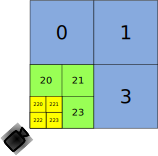
\includegraphics[height=0.17\textheight]{figs/partitioning}}
    \subfigure{}{\includegraphics[height=0.17\textheight]{figs/quadtree_activefront}}
  \end{center}
\caption{In \cite{dupuy2014quadtrees}, a linear quadtree is used to
  maintain a 2D hierarchical partitioning of space.  (Left) presents
  such a partitioning.  A cell is more or less subdivided depending on
  its distance to the camera.  They are also encoded with morton code,
  that identifies each cell with its position relatively to its
  parent.  (Right) shows the corresponding active front in the full
  tree.  This partition is entirely represented by storing the list of
  codes of the gray cells. }
\label{fig_quadtree_partitionning}
\end{figure}




Linear quadtrees or octrees are non-recursive spatial data structure
to represent classical quadtree/octreee trees (see for instance
Gargantini \cite{gargantini1982effective}).  Such structures were
reused by Dupuy \textit{et al.}  \cite{dupuy2014quadtrees} who
presented a solution to handle them efficiently on the GPU.  Linear
quadtrees associate a code to each cell, identifying it by its path to
the root node.  The full tree is thus entirely represented by the list
of its leaves' codes, which removes the recursivity.  In their
implementation, Dupuy \textit{et al.} used Morton codes (Figure
\ref{fig_quadtree_partitionning}).  Those codes store a spatial
position, encoding the location of the cell relatively to its parent.
The final code of a cell is thus the succession of locations between
the cell and the root node.  Therefore, the maximal depth of the tree
depends on the number of quadrants that can be encoded.  In a
quadtree, a cell is divided into $2^2$ quadrants, so encoding one
subdivision requires two bits.  Dupuy \textit{et al.} store for each
cell its Morton code and its depth within the tree.  Therefore, with a
code stored on 32 bits, using 28 bits for the locations and 4 bits for
the depth, the tree is limited to 14 levels.

Dupuy \textit{et al}. used those quadtrees to maintain a 2D
hierarchical space partition.  They thus encode a front of cells
within this tree (Figure \ref{fig_quadtree_partitionning}).  To
determine if a cell is part of the front, they evaluate on each of
them a LoD criterion.  The criterion they chose is view dependent and
thus must be evaluated quickly on the GPU.

During an update, there a three possible operations on a cell: it can
be kept, merged or split.  A merge operation removes the codes of the
children's cells from the list and replaces them with the code of the
parent cell.  A split operation removes the code of a cell replacing
it by the codes of its children.  Therefore, an efficient GPU
implementation relies on the fact that those operations can be done
independently on each cell.  This is true as long as the LoD criterion
is also evaluable independently on each cell.

With this implementation of linear tree, it is possible to maintain a
quadtree on the GPU.  By generalizing this to the octree, it could be
used with the triangulation presented by Lengyel \textit{et al.} to
develop a fully data parallel pipeline.  There is however three
conditions on the LoD criterion.  It must ensure that the extracted
triangles will project onto more than one pixel, to ensure a good
rasterization sampling.  The tree must also stay restricted at all
times as the transition cells of Lengyel \textit{et al.} only patch
cells with a single change in resolution.  Finally, this criterion
must allow to detect if the neighbour of a cell is more subdivided
than the cell itself in a data parallel manner.  This is mandatory to
determine where the transition cells should be inserted.

\todo[inline]{work in progress, cleanup needed}

\subsection{Data parallel and adaptive mesh generation}






\begin{figure}[!htbp]
\centering
\subfigure{}{\includegraphics[width=0.4\linewidth]{mesh_muti_res}}
\subfigure{}{\includegraphics[width=0.4\linewidth]{octree}}
\caption{Isosurface extraction $(a)$ from a  a linear restricted octree
  $(b)$ of a volumetric data.\label{fig:isoexample}}
\end{figure}



\begin{figure}[!htbp]
  \centering
  \includegraphics[width=0.9\textwidth]{figs/pipeline}
  \caption{ This figure summarizes our GPU pipeline. Data buffers are
    represented in green and computations in red. Each computation
    retrieves data from a buffer and fills a new one. }
  \label{fig_pipeline} 
\end{figure}



\section{Interactive Computation on GPU}
\label{sec:inter-visu-gpu}





A {\em cell} is a tuple $(k,x,y,z)$, which represents a region of the space of size $2^k \times
2^k \times 2^k$, characterized by its integer coordinates $x,y,z$,
with $0 \le x < 2^k$, $0 \le y < 2^k$, $0 \le z < 2^k$. Cells forms an
octree decomposition of a cubic space. We use functions Up, Down and
Next to navigate between cells.


\begin{algorithm}
\KwIn{Integers $p,q,r$ \tcp*{the moment orders, with $0 \le p+q+r \le 2$}}
\KwIn{Integer $k$ \tcp*{$(2^k)^3$ is the size of the digital shape image}}
\KwIn{Mipmap $V$ \tcp*{array of $k+1$ images of sizes $(2^k)^3,  (2^{k-1})^3, \ldots,  1^3$}}
\KwIn{Integers $x_0,y_0,z_0$, Real $r$ \tcp*{Ball radius $r$ and center $(x_0,y_0,z_0)$}}
\KwOut{Real $m$ \tcp*{estimation of the $p,q,r$-moment of $X \cap B_r(x_0,y_0,z_0)$}}
\KwData{Cell $c :=  (k,0,0,0)$ \tcp*{Starts from biggest cell}}
\KwData{Integer $n := 2^k$ \tcp*{Size of each cell}}
\KwData{Real $d,\delta,l$ \tcp*{variables for intermediate computations}}
\Begin{
    m := 0 \;
    \Repeat{$c[0] = k$}{
      \tcp{Distance between cell and ball centers}
      $d := \frac{1}{2}\| 2^k(2c[1]+1,2c[2]+1,2c[3]+1) - (2x_0+1,2y_0+1,2z_0+1) \|_2$\;
      $\delta := \frac{\sqrt{3}}{2}2^{c[0]}$ \tcp*{half-length of cell diagonal}
      \If(\tcp*[f]{Is it a unit cell ?}){$c[0] = 0$}{
        \If(\tcp*[f]{Is cell center inside ball ?}){$d^2 \le r^2$}{
          $m := m + V[c] * (2^k c[1])^p * (2^k c[2])^q * (2^k c[3])^r$ \;
        }
        $c := \textsc{Next}(c)$ \tcp*{Go to next cell}
      } \Else{
        $l := \max(r-\delta,0)$\;
        \If(\tcp*[f]{Is cell completely inside ball ?}){$d^2 < l^2$}{
          $m := m + V[c] * (2^k c[1])^p * (2^k c[2])^q * (2^k c[3])^r$\;
          $c := \textsc{Next}(c)$ \tcp*{Go to next cell}
        }\ElseIf(\tcp*[f]{Is cell outside ball ?}){$d^2 > (r+\delta)^2$}{
          $c := \textsc{Next}(c)$ \tcp*{Go to next cell}
        }\lElse(\tcp*[f]{Go to a finer cell}){$c := \textsc{Down}(c)$}
      }
    }
    \Return{m}\;
  }
  \caption{Derecursified hierarchical algorithm for computing the
    $p,q,r$-moment of set $X \cap B_r(x_0,y_0,z_0)$, given a mipmap
    $V$ that represents the volume of a shape $X$ in each cell, and
    ball parameters $x_0,y_0,z_0,r$.}
\end{algorithm}

\begin{function}
  \caption{Up( Cell $c$ ) : Cell}
  \Return{Cell( $c[0]+1$, $c[1]/2$, $c[2]/2$, $c[3]/2$ )}
\end{function}
\begin{function}
  \caption{Down( Cell $c$ ) : Cell}
  \Return{Cell( $c[0]-1$, $c[1]*2$, $c[2]*2$, $c[3]*2$ )}
\end{function}
\begin{function}
  \caption{Next( Cell $c$ ) : Cell}
  \lWhile{$\mathrm{Odd}(c[1])$ and $\mathrm{Odd}(c[2])$ and $\mathrm{Odd}(c[3])$}{$c := \mathrm{Up}(c)$}
  \lIf{$\mathrm{Even}(c[1])$}{$c[1] := c[1]+1$}
  \Else{$c[1] := c[1] - 1$\;
    \lIf{$\mathrm{Even}(c[2])$}{$c[2] := c[2]+1$}
    \Else{$c[2] := c[2] - 1$\;
      $c[3] := c[3]+1$}
  }
  \Return{c}
\end{function}


\section{Experiments}
\label{sec:experiments}



\section{Conclusion and Discussion}
\label{sec:discussion}



\bibliographystyle{splncs03}
\bibliography{ictv}
\end{document}
